% \documentclass[11pt, paper=a4, oneside]{scrartcl}
\documentclass{article}

% \usepackage{mathtools}

\usepackage{arsclassica}

\usepackage{minted}
\usemintedstyle{friendly}
\newmintedfile[pycode]{python}{
	frame=single,
	framesep=2mm,
	baselinestretch=1,
	fontsize=\footnotesize
}

\usepackage{graphicx}
\graphicspath{{gfx/}}

\addbibresource{Bibliography.bib}

\usepackage{setspace}
\usepackage{siunitx}
% \onehalfspacing

\title{Sorting sentiments of hotel reviews through machine learning}
\author{Darren Yap \and Tan Jia He \and Fu Jinghang}
\date{2024}

% start the document!
\begin{document}
\pagestyle{scrheadings}
% \renewcommand{\sectionmark}[1]{\markright{\spacedlowsmallcaps{#1}}}

\maketitle
\tableofcontents

% ** abstract **
\begin{abstract}
	\noindent
	Hotels depend on tourists to survive. They gather consumer opinions via customer
	reviews to improve their services. This project used sentiment analysis---the
	process of determining the emotional tone of text---to quantify consumers'
	opinions on hotels, and predicted the overall sentiment of hotel reviews.
	International hotel reviews in English were split into individual words,
	assigning each word a score based on its relative intensity. The sentiment
	makeup of the review dataset was highlighted and the most frequent tokens were
	identified. Two machine learning models---a logistic regression model and a random
	forest classifier---were also constructed to predict the overall sentiment of a
	review. It was shown that the models were capable of predicting the overall
	sentiment of hotel reviews. This project highlights the possibility of using
	sentiment analysis models to create applications that allow customers to better
	understand the perceived quality of a hotel and potentially combat review fraud---the
	the dishonest practice of manipulating false reviews to boost a hotel's ratings.
\end{abstract}

\section{Introduction}
After the Singapore government relaxed travel restrictions due to COVID--19,
there has been a recent increase in the number of tourists travelling in and out of Singapore.
As such, hotels have seen a rise in the number of prospective tourists to be housed,
and this may encourage an increase in the number of reviews hotels may receive.

Today, it is common to use social networks, messengers, and review websites
to receive data from customer opinions. This is especially true for hotels,
where previous occupants may evaluate the hotel on several factors through their
reviews---be it cleanliness, facilities, location and convenience, etc.
These come in two forms---a quantitative review (based on stars, diamonds,
hearts, etc.) and a more qualitative review through text.

However, quantitative reviews do not always paint the full picture of customers'
opinions towards a certain hotel. Though it is certainly helpful to have a more
objective rating system using numerical scores, eg. the Department of Tourism
grading system in the Philippines, or the European Hotelstars Union system,
these are given by customers subjectively and do not reflect the reasons for
customers giving the rating. There is also evidence of manipulation of ratings
by hotel management itself, where hotels may be compelled to forge positive or
negative ratings to bias the overall rating. This made up \qty{2.1}{\percent}
of the 66 million reviews submitted to TripAdvisor in \citeyear{tripadvisor}.
Therefore, we propose using sentiment analysis to extract customers' true
feedback on hotels instead.

% \section{Objectives and Research Questions}
% \subsection{Objectives}
% \begin{enumerate}
% 	\item To run sentiment analysis on individual words and quantify them on a numerical scale
% 	\item To run sentiment analysis on paragraphs and quantify them on a numerical scale
% 	\item To use sentiment analysis on hotel reviews to determine consumers' overall opinions of hotels
% \end{enumerate}

% \subsection{Research Questions}
% \begin{enumerate}
% 	\item How could we quantify the sentiments of individual words on a numerical scale?
% 	\item How could we quantify the sentiments of paragraphs on a numerical scale?
% 	\item How could we use tokens in hotel reviews to predict the overall sentiment of the review?
% \end{enumerate}

% \subsection{Fields of Math}
% \begin{itemize}
% 	\item Statistics and probability theory
% \end{itemize}

% \subsection{Terminology}
% Below is a listing of the terminology, mostly pertaining to sentiment
% analysis, used in this report.

% % update this!
% % \begin{table}[htpb]
% % \caption{Terminology used in this report.}
% % \label{tab:terms}
% \begin{center}
% 	\begin{longtable}{|p{.3\textwidth}|p{.7\textwidth}|}
% 		\hline
% 		\bf{Term}                        & \bf{Definition}                                                                                                                                                                                                                                     \\
% 		\hline
% 		Sentiment analysis               & Process of determining the emotional tone of text                                                                                                                                                                                                   \\
% 		\hline
% 		Token                            & A unit of meaning (usually a word) that carries sentiment                                                                                                                                                                                           \\
% 		\hline
% 		Tokenise                         & To split a piece of text up into its constituent tokens, to be used for further analysis.                                                                                                                                                           \\
% 		\hline
% 		Lemmatise                        & To sort, so as to group together, inflected or variant forms of the same word, eg. `watching', `watchful', and `watched'                                                                                                                            \\
% 		\hline
% 		Stop words                       & Tokens that carry little meaning during sentiment identification, such as `is', `I', `that', etc.; that should be filtered out before the processing of text                                                                                        \\
% 		\hline
% 		Lexicon                          & A dictionary that maps singular tokens to a category of sentiments or sentiment scores                                                                                                                                                              \\
% 		\hline
% 		Polarity                         & Whether a piece of text is positive, negative or neutral in sentiment                                                                                                                                                                               \\
% 		\hline
% 		Bipartite sentiment              & Sentiment which is grouped into two categories, usually positive and negative                                                                                                                                                                       \\
% 		\hline
% 		Tripartite sentiment             & Sentiment which is grouped into three categories, usually positive, negative and neutral                                                                                                                                                            \\
% 		\hline
% 		Sentiment score                  & A number that shows the overall sentiment of a token or a piece of text                                                                                                                                                                             \\
% 		\hline
% 		Lexicon-based sentiment analysis & A method of sentiment analysis which sorts tokens into categories, aided by a lexicon, then calculates the overall sentiment score of a piece of text                                                                                               \\
% 		\hline
% 		Corpus-based sentiment analysis  & A method of sentiment analysis which relies on the co-occurrences of tokens within a piece of text itself, rather than relying on an external lexicon                                                                                               \\
% 		\hline
% 		True positive                    & A prediction made by a machine learning model that \bf{correctly} matches up with its intended value, e.g. should a review’s sentiment be positive and a model predicts its sentiment to be positive, the model has made a true positive prediction \\
% 		\hline
% 		False positive                   & A prediction made by a machine learning model that \bf{incorrectly} reflects its intended value, e.g. should a review’s sentiment be negative and a model predicts its sentiment to be positive, the model has made a false positive prediction     \\
% 		\hline
% 	\end{longtable}
% \end{center}
% % \end{table}

% \section{Literature Review}
% Sentiment analysis is a field of study which utilises computational methods to analyse text,
% and then categorises the text, usually into three main polarities---positive, neutral
% and negative. It has broad applications which range from determining consumers' opinion in
% sales and product analysis, to competitor research in marketing, and even detecting public
% opinion in social media monitoring. Sentiment analysis will be used in this project to
% analyse hotel occupants' reviews, and also determine the most significant upsides
% and downsides of each hotel, without interference from human bias.

% The stock market opinion of StockTwits communities
% of expert investors was predicted. Sentiment analysis was used in a Deep Learning model to extract
% sentiment from Big Data. A Pearson Correlation Coefficient combined the linear correlation
% between users' sentiment and future stock prices, which
% proved the accuracy of user sentiment to be \qty{53}{\percent}.
% It was concluded that convolutional neural networks (CNN), a type of Deep Learning
% artificial neural network, was able to predict stock market movement based on sentiment (\cite{stock}).

% Using the social networking site Twitter,
% Filipinos' sentiment in response to the Philippine government's efforts
% at tackling COVID--19 was determined (\cite{twitter}), specifically the implementation of vaccination. Natural
% Language Processing (NLP) techniques such as sentiment analysis were used to
% extract sentiment from text in the English and Filipino languages, which was used to
% train a Naïve-Bayes model. A confusion matrix was produced, representing the
% prediction accuracy of the Naïve-Bayes model (\qty{81.77}{\percent}) at classifying
% sentiment into positive, neutral and negative categories. It was concluded that
% sentiment analysis towards COVID-19 vaccines were very accurate, even helping the
% Philippine government better conduct budget planning and coordinate COVID-19 efforts.

% % cite
% Tourism quality in Spain was analysed (\cite{spain}) by
% extracting sentiment from reviews by Chinese people on the tourism
% social networking sites Baidu Travel, Ctrip, Mafengwo, and Qunar.
% Two sentiment analysis methods, lexicon-matching and corpus-based machine
% learning methods, were used. These methods allow the processing of
% unstructured text of comparatively longer lengths. Clustered data
% visualisation categorised aspects of Spanish tourism into positive
% and negative groups, with the majority residing with positive sentiment.
% It was concluded that sentiment analysis can be used to improve tourism
% quality and sustainability decision-making.

% SentiStrength, a tool for lexical sentiment analysis---sentiment analysis done
% on short, low quality texts---was used to study emotions expressed in GitHub
% commit comments of different open-source projects (\cite{github}).
% Their method involved assigning scores to each word, then calculating the net
% score for each comment. SentiStrength splits each comment into snippets, assigns
% each a score by computing the maximum and minimum scores of the sentences it contains.
% Following which, the average of the positive and negative scores is taken as the
% sentiment score of the entire commit. This study showed that Java projects warranted
% more negative comments, and projects which had more distributed teams tended
% to have a higher positive sentiment.

% In conclusion, the literature reviewed showed many possible applications
% of sentiment analysis in quantifying the underlying emotion of feedback
% on online platforms. Lexicon-based sentiment analysis, which assigns each
% word a sentiment, then calculates a sentence's total sentiment score, can
% be used, due to its simplicity in implementation, and the availability of
% many open-source sentiment lexicons. In addition, sentiment categorisation
% using lexicon-based sentiment analysis makes accurate predictions upwards of
% \qty{70}{\percent} of the time (\cite{khoo}). SentiStrength would also be useful for
% detecting sentiment from hotel reviews which are usually short in length quickly
% and efficiently, optimising the process of extracting sentiment from tourists'
% reviews of hotels. Using SentiStrength for sentiment generation is also
% rather accurate, generating both positive and negative sentiments with more
% than \qty{60}{\percent} accuracy (\cite{thelwall}). Therefore, the strategies listed % TODO cite!
% above could be adopted or emulated on a smaller scale for this project.

% \section{Methodology}

% \subsection{Research Question 1}
% \it{How could we quantify the sentiments of individual words on a numerical scale?}

% A valence dictionary, which maps individual tokens to a single
% sentiment score, was sourced for. After collecting an open-source dataset
% of international hotel reviews in English, the reviews were tokenised:
% split into its individual tokens. Each word was assigned a sentiment score,
% and word clouds were generated to display the most frequent positive and
% negative tokens in the dataset.

% \subsection{Research Question 2}
% \it{How could we quantify the sentiments of paragraphs on a numerical scale?}

% SentiStrength was used (\cite{github}) to evaluate the total positive % TODO cite!
% and negative sentiments of each review. Two scores for each review were expected:
% the total positive sentiment score (in the range \([1, 5]\)) and the total negative
% sentiment (in the range \([-5, -1]\)). This is similar to how GitHub commit
% messages were classified.

% To classify the sentiments of each review into one of three categories:
% positive (\(1\)), neutral (\(0\)) and negative (\(-1\)), the two scores of each review
% were added. We define the following, where \(k\) represents the polarity of a review,
% and \(S_+\) and \(S_-\) represent the positive and negative sentiment scores of a review:

% \begin{equation}
% 	k = \begin{cases}
% 		1  & \text{if } S_+ + S_- > 0 \\
% 		0  & \text{if } S_+ = S_-     \\
% 		-1 & \text{if } S_+ + S_- < 0 \\
% 	\end{cases}
% 	\label{eq:polarity}
% \end{equation}

% \subsection{Research Question 3}
% \it{How could we use tokens in hotel reviews to predict the overall sentiment of a review?}

% \subsubsection{Logistic Regression Model}
% A \bf{logistic regression model} was constructed to classify the reviews collected into
% two categories: those with a net positive sentiment and those with a net negative sentiment.
% The reviews were split into training, testing and prediction sets.

% Each review was tokenised and lemmatised. A feature vector for each review was
% then constructed, which shows how often each word occurs in the particular review---the
% term frequencies for each word, where \(\text{tf}(t,d)\) represents the relative term frequency of
% token \(t\) in review \(d\):

% \begin{equation}
% 	\text{tf}(t,d) = \frac{f_{t,d}}{\sum_{t'\in d}^{}f_{t',d}}
% 	\label{eq:tf}
% \end{equation}

% where \(f_{t,d}\) is the raw count of a token \(t\) in review \(d\). The denominator of the above
% function is simply the total number of tokens in review \(d\).

% To evaluate the relevance of a token in determining the overall sentiment of the
% review, the \bf{term frequency-inverse document frequency} (\it{tf-idf}) is found, where:

% \begin{equation}
% 	\text{tfidf}(t,d,D) = \text{tf}(t,d)\cdot\lg\frac{N}{1+\left|\left\{d\in D : t\in d\right\}\right|}
% 	\label{eq:tfidf}
% \end{equation}

% also where \(N\) is the total number of documents in the set of reviews, and
% \(\left|\left\{d\in D : t\in d\right\}\right|\) is the number of reviews where
% the token \(t\) occurs. \(1\) is added to the denominator to prevent a
% division-by-zero scenario, should the token not appear in the review at all.

% A conventional \bf{sigmoid function} was used to evaluate the probability
% of a review carrying a net positive sentiment, a value from 0 to 1:

% \begin{equation}
% 	h_\theta(x) = \frac{1}{1+e^{-{\left(\beta_0+\beta_1x\right)}}}
% 	\label{eq:sigmoid}
% \end{equation}

% where \(h_\theta(x)\) is the probability of the net sentiment of a review being positive, and
% \(\beta_0+\beta_1x\) is a linear function of \it{tf-idf} \(x\).

% The error in the logistic regression model is given by the cost function:
% \begin{equation}
% 	\text{cost}\left(h_\theta\left(x\right),y\right) = \begin{cases}
% 		-\log\left(h_\theta\left(x\right)\right)   & \text{if } y = 1 \\
% 		-\log\left(1-h_\theta\left(x\right)\right) & \text{if } y = 0
% 	\end{cases}
% \end{equation}
% where \(y\) is the predicted output (a positive or negative outcome) for every \(x\).

% Lastly, the model used gradient descent to minimise this cost.

% After the model was constructed, predictions were made using the aforementioned
% prediction dataset. Precision-recall and receiver operating characterstic curves
% were plotted to evaluate the precision of the model,
% and how well the model distinguishes between false positive and true positive predictions.
% For the precision-recall curve, precision (\(P\)) is defined as:

% \begin{equation}
% 	P = \frac{T_p}{T_p + F_p}
% 	\label{eq:prec}
% \end{equation}

% where \(T_p\) is the number of true positives and \(F_p\) is the number of false positives.

% Recall (\(R\)) is defined as:

% \begin{equation}
% 	R = \frac{T_p}{T_p + F_n}
% 	\label{eq:recall}
% \end{equation}

% where \(F_n\) is the number of false negative predictions.

% As for the receiver operating characteristic curve, the rate
% of true positive predictions (\(\text{TPR}\)) was plotted over the rate of
% false positive predictions (\(\text{FPR}\)), where

% \begin{equation}
% 	\text{TPR} = \frac{T_p}{T_p + F_n}
% 	\label{eq:TPR}
% \end{equation}

% and
% \begin{equation}
% 	\text{FPR} = \frac{F_p}{F_p + T_n}
% 	\label{eq:FPR}
% \end{equation}

% where \(F_p\) is the number of false positive predictions
% and \(T_n\) is the number of true negative predictions.

% \subsubsection{Random Forest Classifier}
% A \bf{random forest classifier} was also constructed
% to predict whether hotel reviews carry a net positive or
% negative sentiment. The individual positive and negative sentiment
% scores generated by SentiStrength were used as \it{features},
% fed into the random forest classifier.

% Similarly to the logistic regression model,
% vector representations for each review were generated,
% with each token's corresponding \it{tf-idf} values evaluating the
% relative importance of each token in determining the sentiment
% of each review. By using the \it{tf-idf} values of each token as
% the independent variable and its corresponding sentiment polarity
% as the dependent variable, the classifier was trained.

% As above, precision-recall and receiver operating characteristic
% graphs were plotted to evaluate the precision of the random forest
% classifier, as well as how well the model distinguishes between true
% positive and false positive predictions.

% \section{Results}
% \subsection{RQ1: Token-Based Sentiment Analysis}
% After tokenising English hotel reviews from the dataset of international hotel reviews,
% the \it{Afinn} lexicon was used to assign each token a single numerical score. This
% score ranges from \([-5, -1]\) for negative tokens, and \([1, 5]\) for positive tokens,
% with the magnitude representing the degree of negativity or positivity the token holds.
% Tokens with a sentiment score of \(0\) carry neutral sentiment.

% \begin{figure}[htpb]
% 	\begin{center}
% 		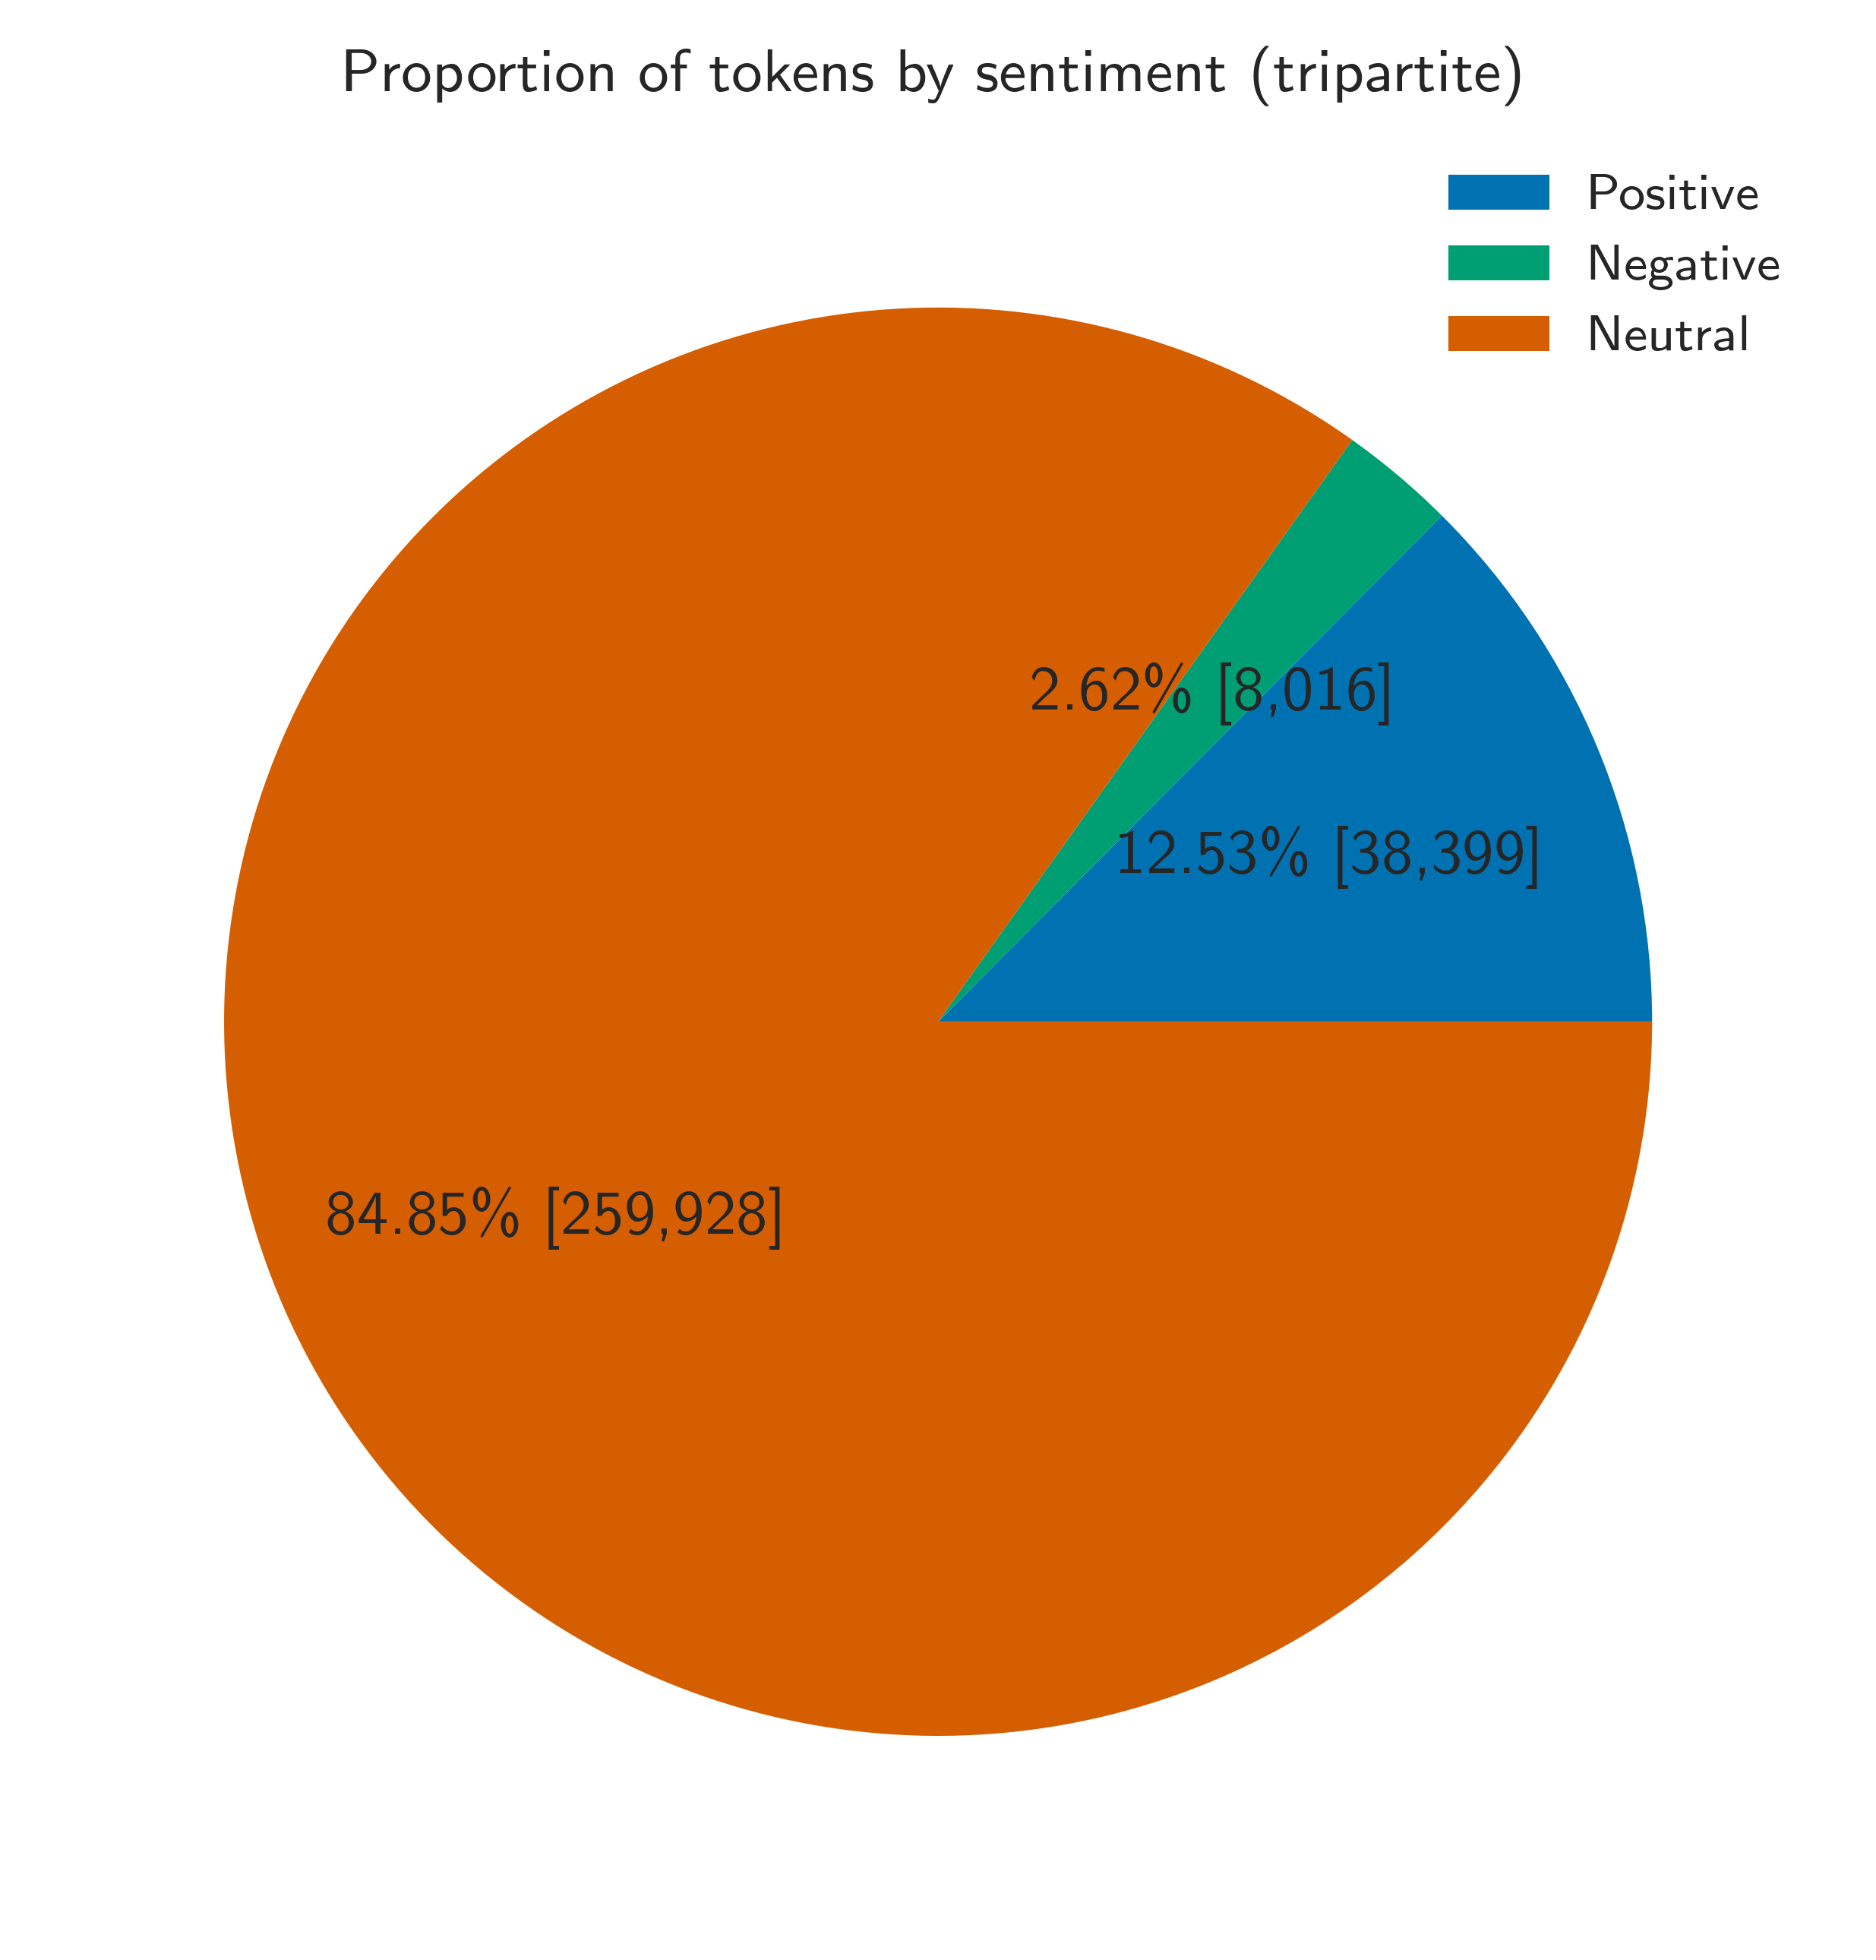
\includegraphics[width=0.5\textwidth]{rq1/pie_tripartite.png}
% 	\end{center}
% 	\caption{Proportion of tokens by sentiment (positive v. negative v. neutral)}
% 	\label{fig:reviews-pie1}
% \end{figure}

% \begin{figure}[htpb]
% 	\begin{center}
% 		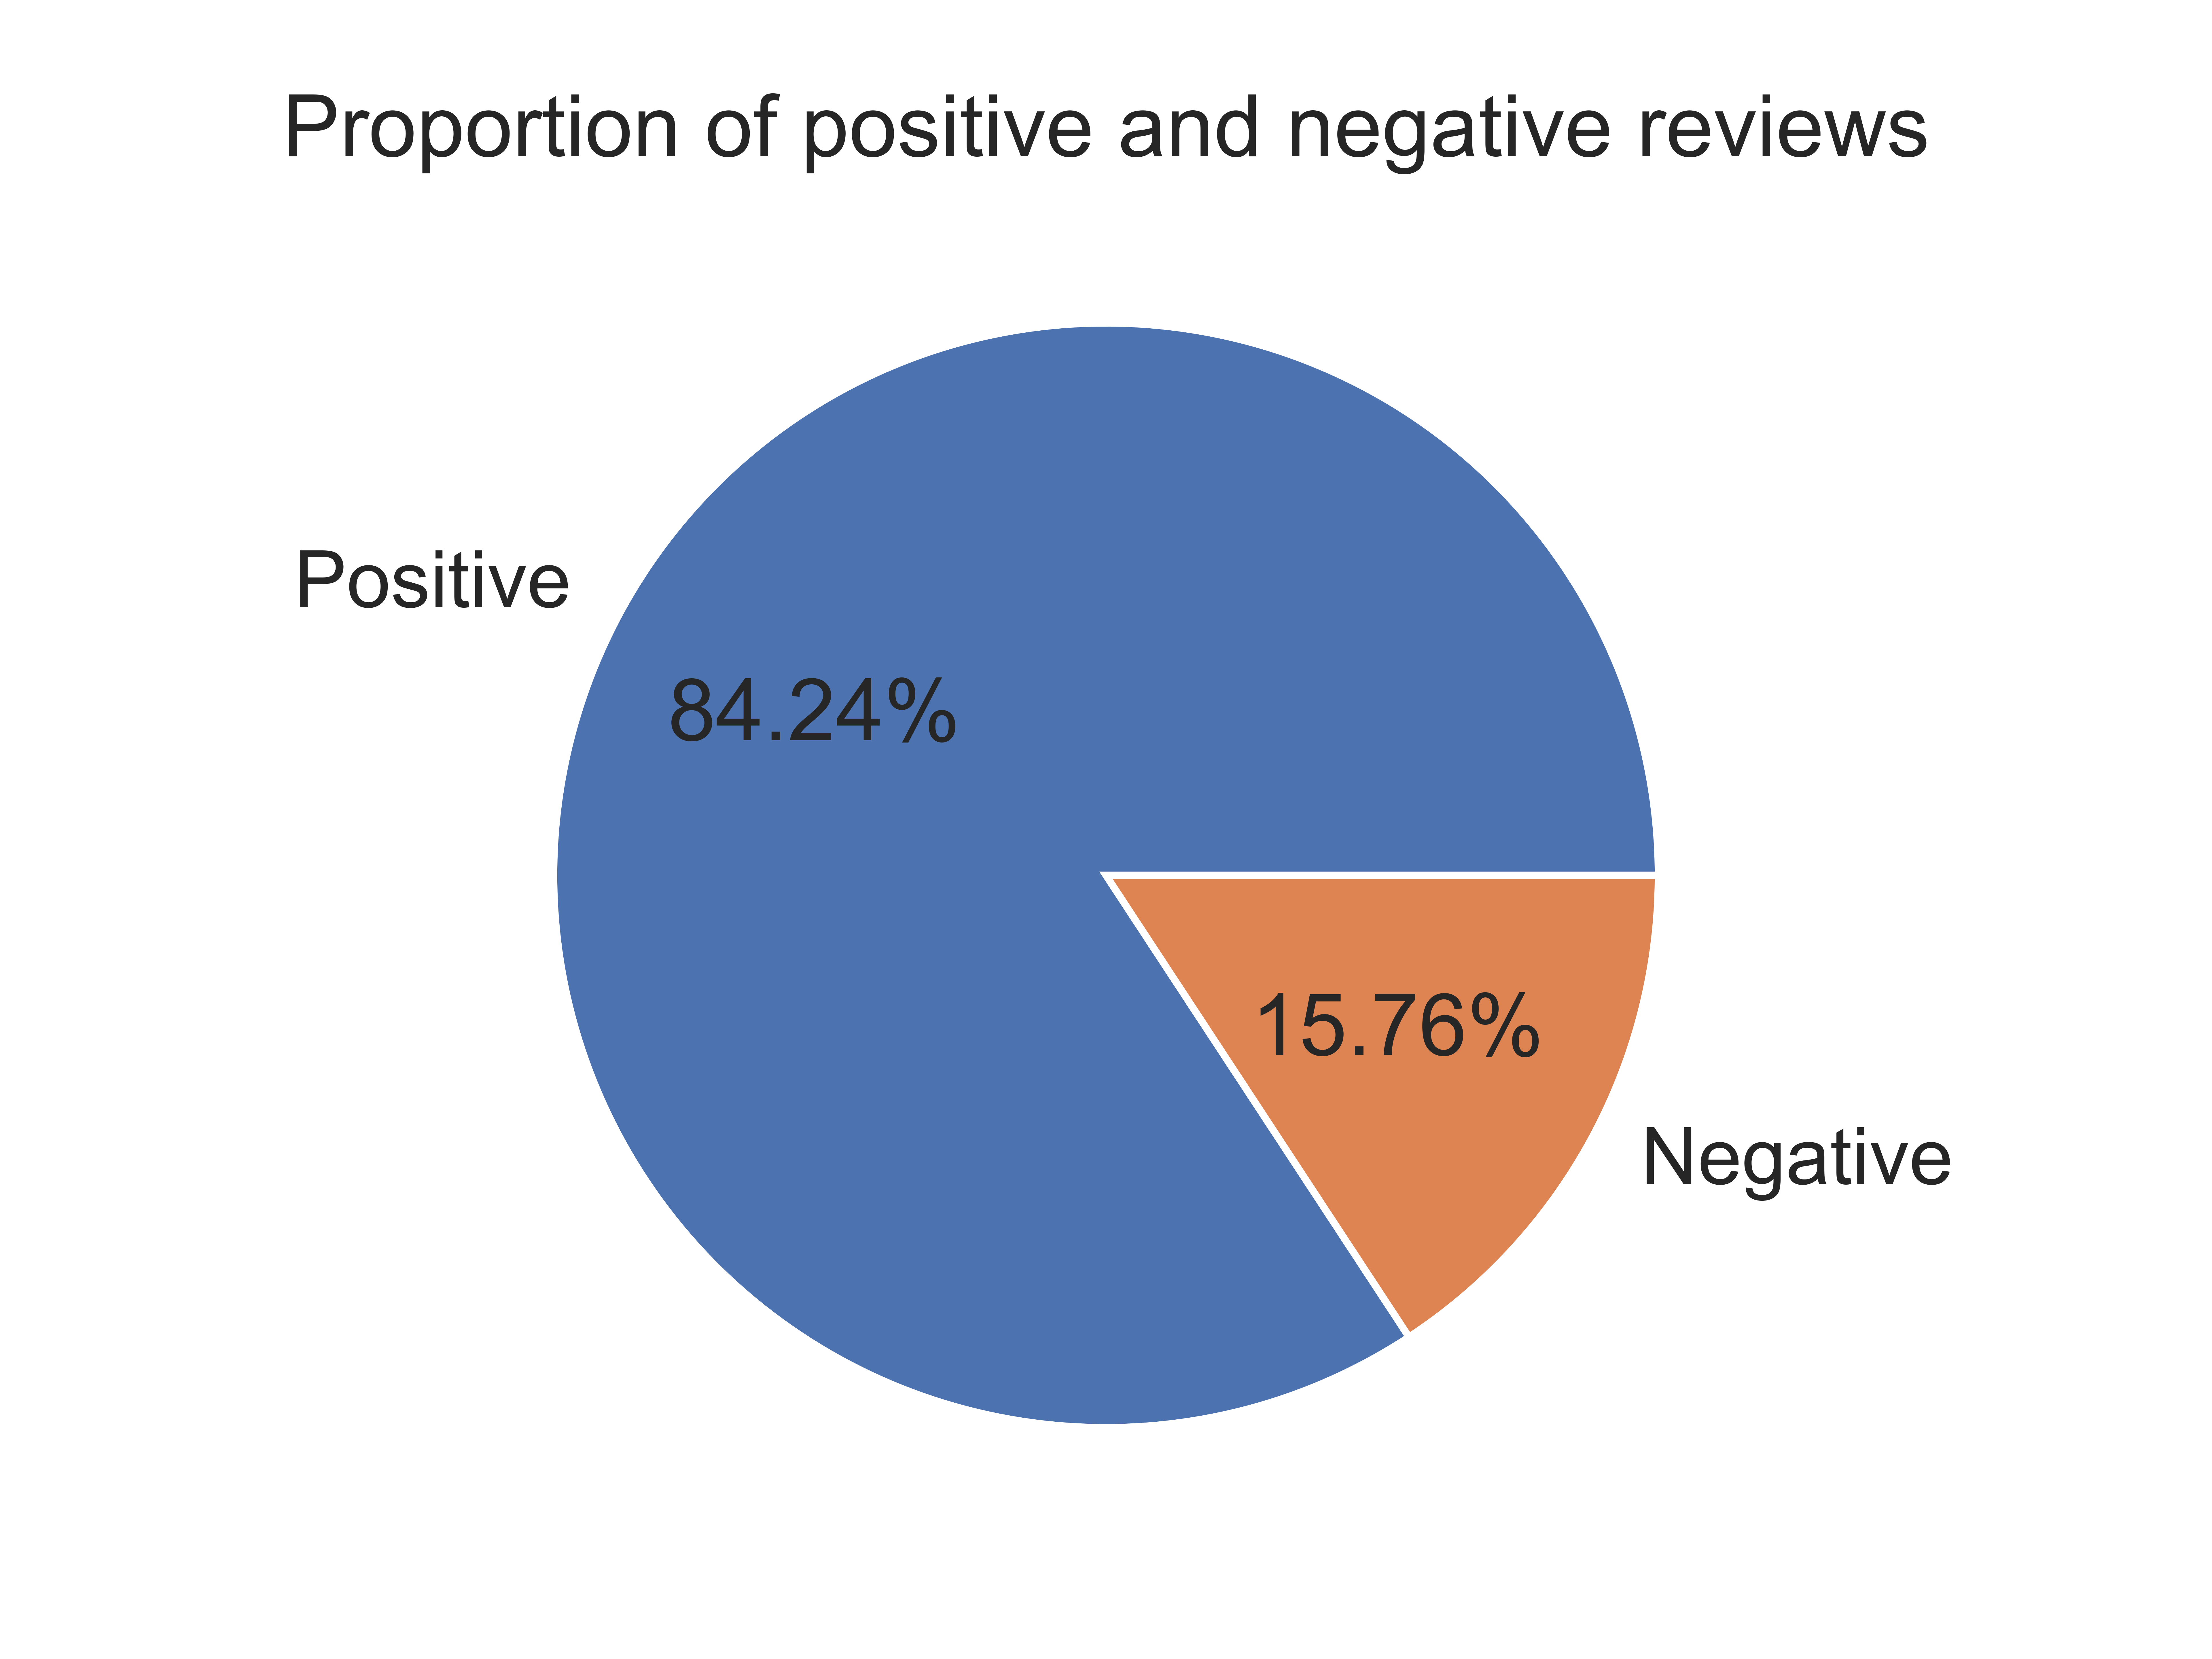
\includegraphics[width=0.6\textwidth]{rq1/pie_bipartite.png}
% 	\end{center}
% 	\caption{Proportion of tokens by sentiment (positive v. negative)}
% 	\label{fig:reviews-pie2}
% \end{figure}

% While it is observed that there are more tokens with positive sentiment than
% their negative counterparts, the vast majority of tokens in
% Figure~\ref{fig:reviews-pie1} hold a neutral sentiment (\qty{84}{\percent}),
% due to the presence of many standalone tokens that do not express opinion,
% eg. \it{hotel}, \it{food}, and \it{visit}.

% Word clouds of positive and negative tokens were also produced.
% The more frequently a token appears in either the word clouds of
% net positive or net negative hotel reviews (that carries either a positive
% or negative sentiment based on the lexicon), the larger the word in the word cloud,
% hence the more significant the token, and the better it represents the positive
% or negative features of a hotel.

% \begin{figure}[htpb]
% 	\begin{center}
% 		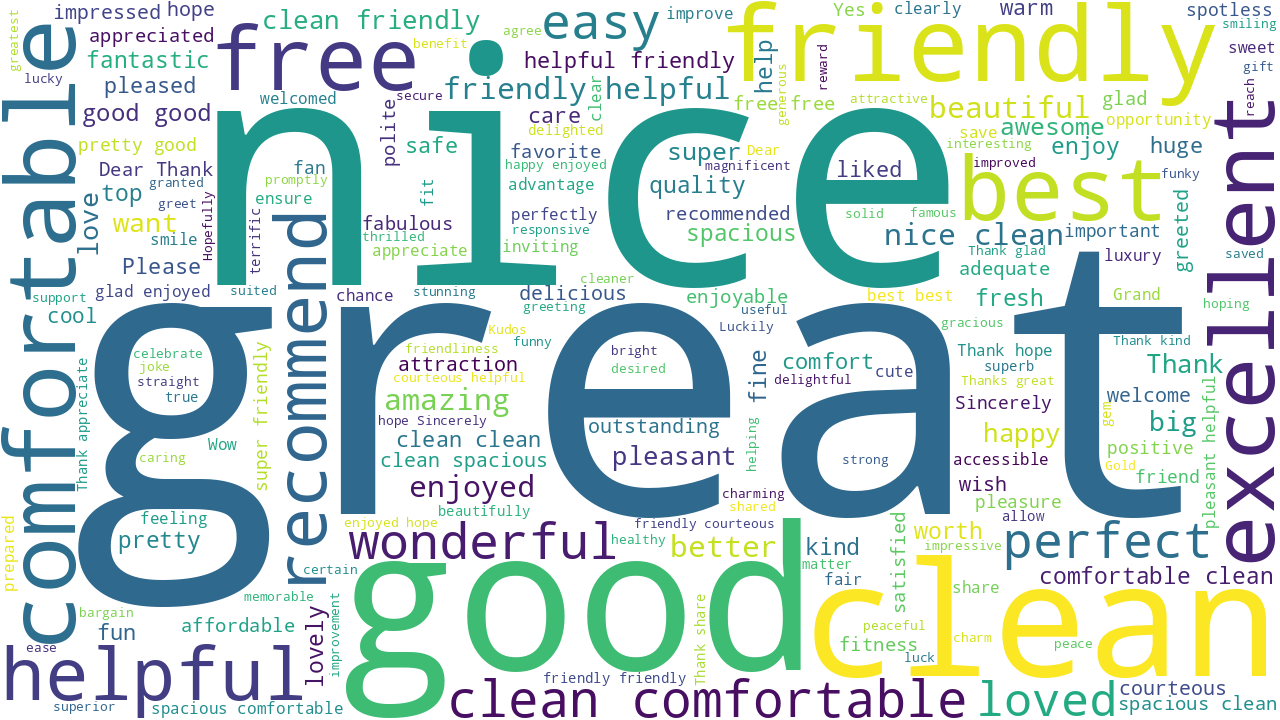
\includegraphics[width=0.75\textwidth]{rq1/wordcloud_pos.png}
% 	\end{center}
% 	\caption{Word cloud (positive tokens)}
% 	\label{fig:wordcloud-pos}
% \end{figure}

% \begin{figure}[htpb]
% 	\begin{center}
% 		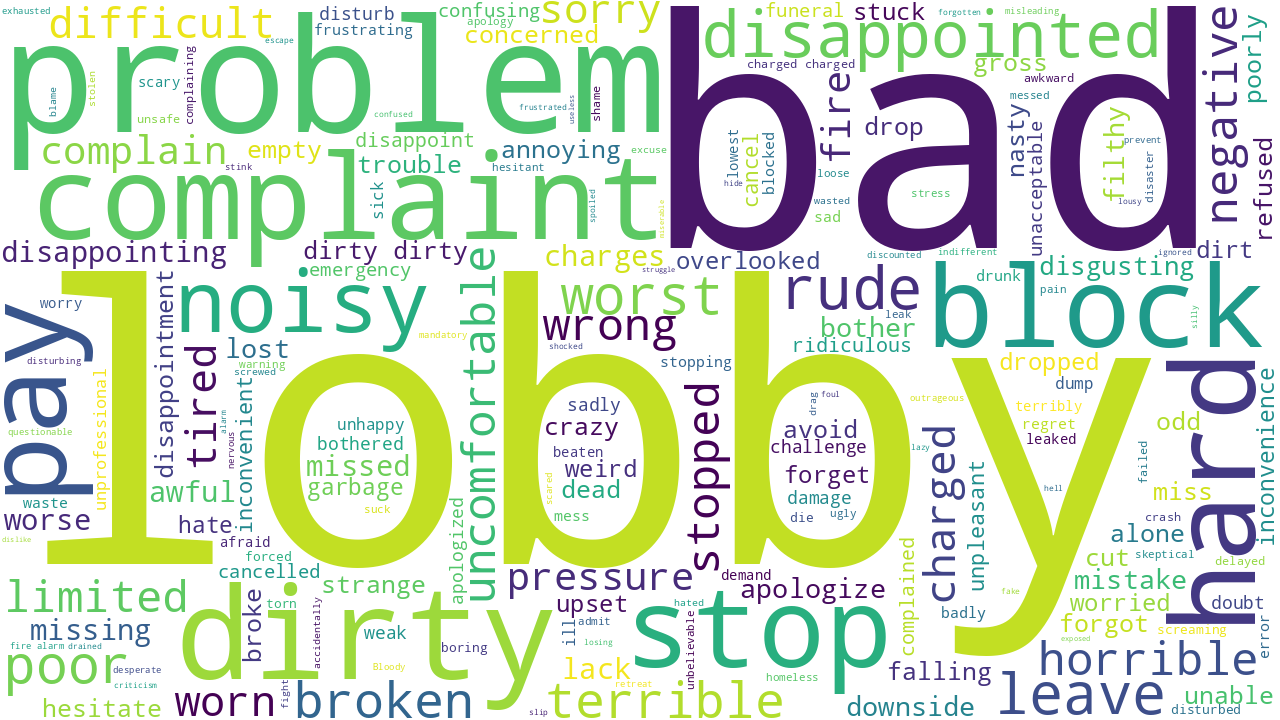
\includegraphics[width=0.75\textwidth]{rq1/wordcloud_neg.png}
% 	\end{center}
% 	\caption{Word cloud (negative tokens)}
% 	\label{fig:wordcloud-neg}
% \end{figure}

% Words of positive sentiment of greater size in the word cloud,
% such as \it{great} and \it{nice}, are more prominent traits that tourists associate
% with their experience at the hotels, while words of negative sentiment, such as \it{lobby}
% and \it{bad}, are more common among customers with dissatisfaction towards their hotels.

% \subsection{RQ2: Review-Based Sentiment Analysis}
% SentiStrength was used to generate two scores for each review: a positive and
% negative score, initialised to \(1\) and \(-1\) respectively. As the reviews were analysed
% on a token-by-token basis, the polarity of the token determined which score it contributed
% to. The individual score of the token would then be added to either the net positive or
% net negative score of the review. To illustrate, the token \it{friendly} would contribute
% a positive score of \(1\), while the token \it{amazing} would contribute a positive score of \(2\),
% because it holds a stronger positive connotation. In addition, the use of punctuation was
% considered as well---exclamation marks for emphasis contributed to either the positive or
% negative score, depending on the sentiments of the tokens before and after them.

% The positive and negative scores determined the extent to which the review was positive
% or negative. All positive scores were in the range \([1, 5]\), and the negative scores were
% in the range \([-5, -1]\).

% \begin{figure}[htpb]
% 	\begin{center}
% 		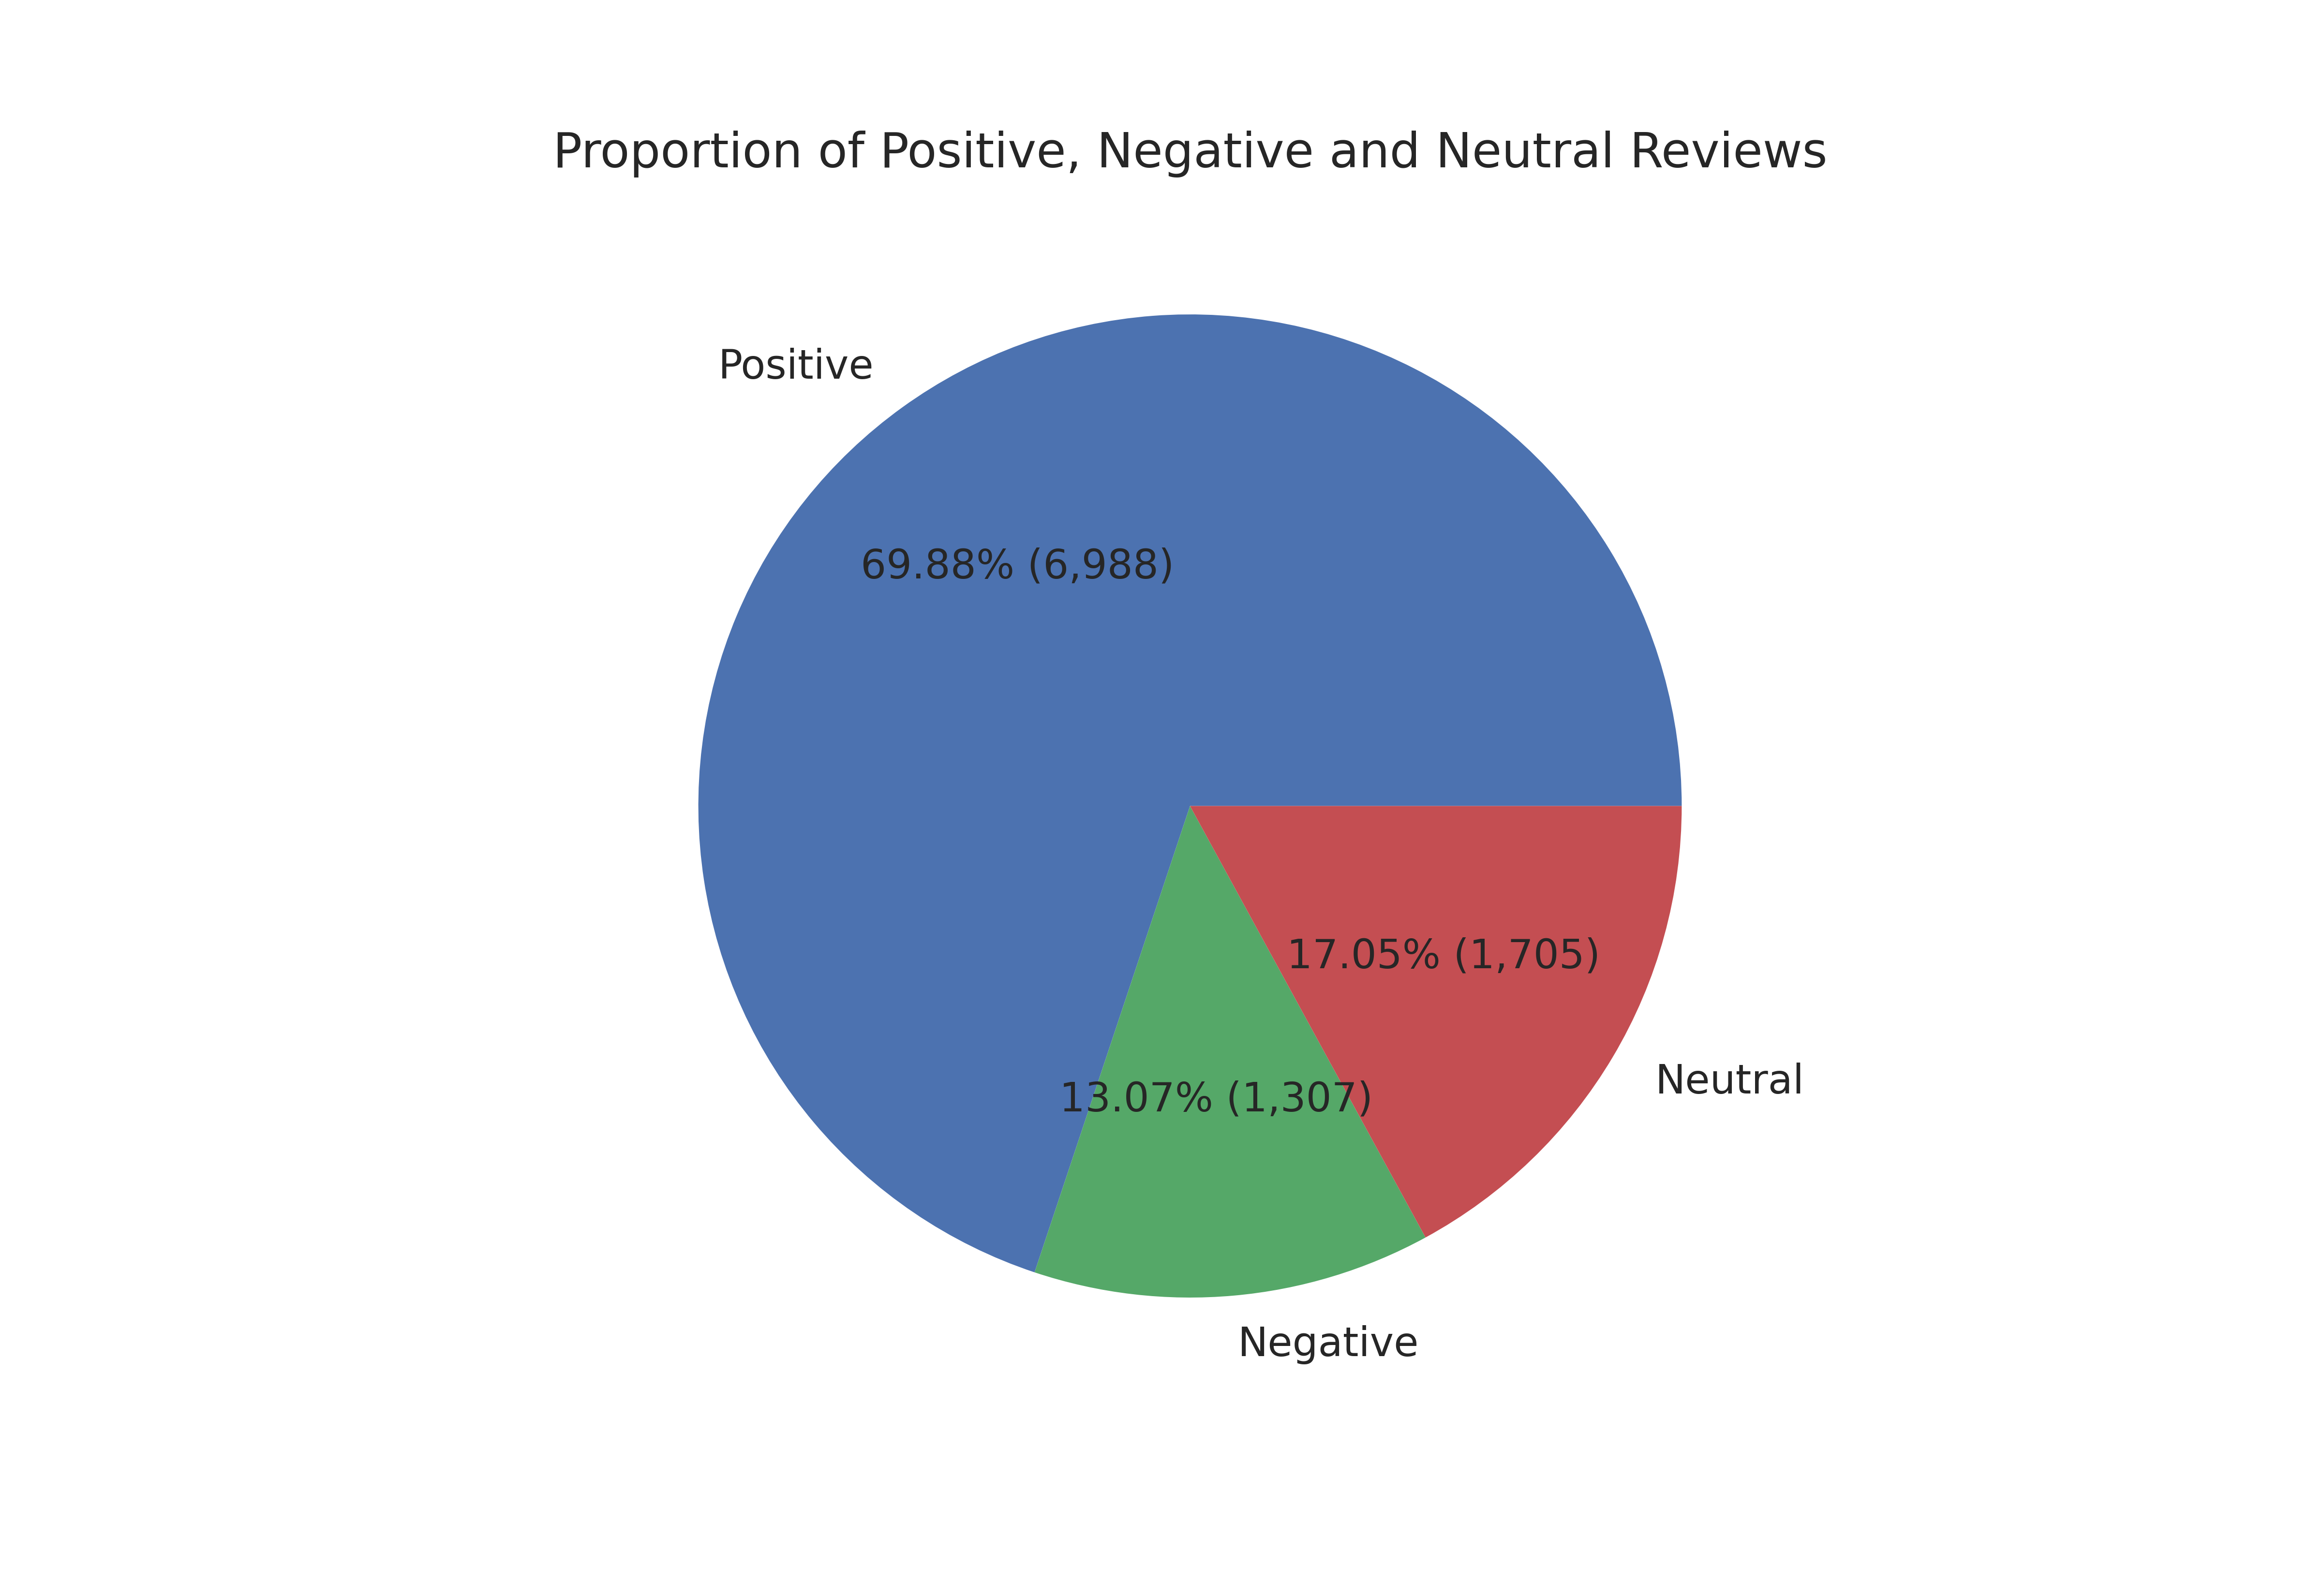
\includegraphics[width=0.6\textwidth]{rq2/pie_chart_3part.png}
% 	\end{center}
% 	\caption{Proportion of reviews (positive v. negative v. neutral)}
% 	\label{fig:reviews-pie3}
% \end{figure}

% \begin{figure}[htpb]
% 	\begin{center}
% 		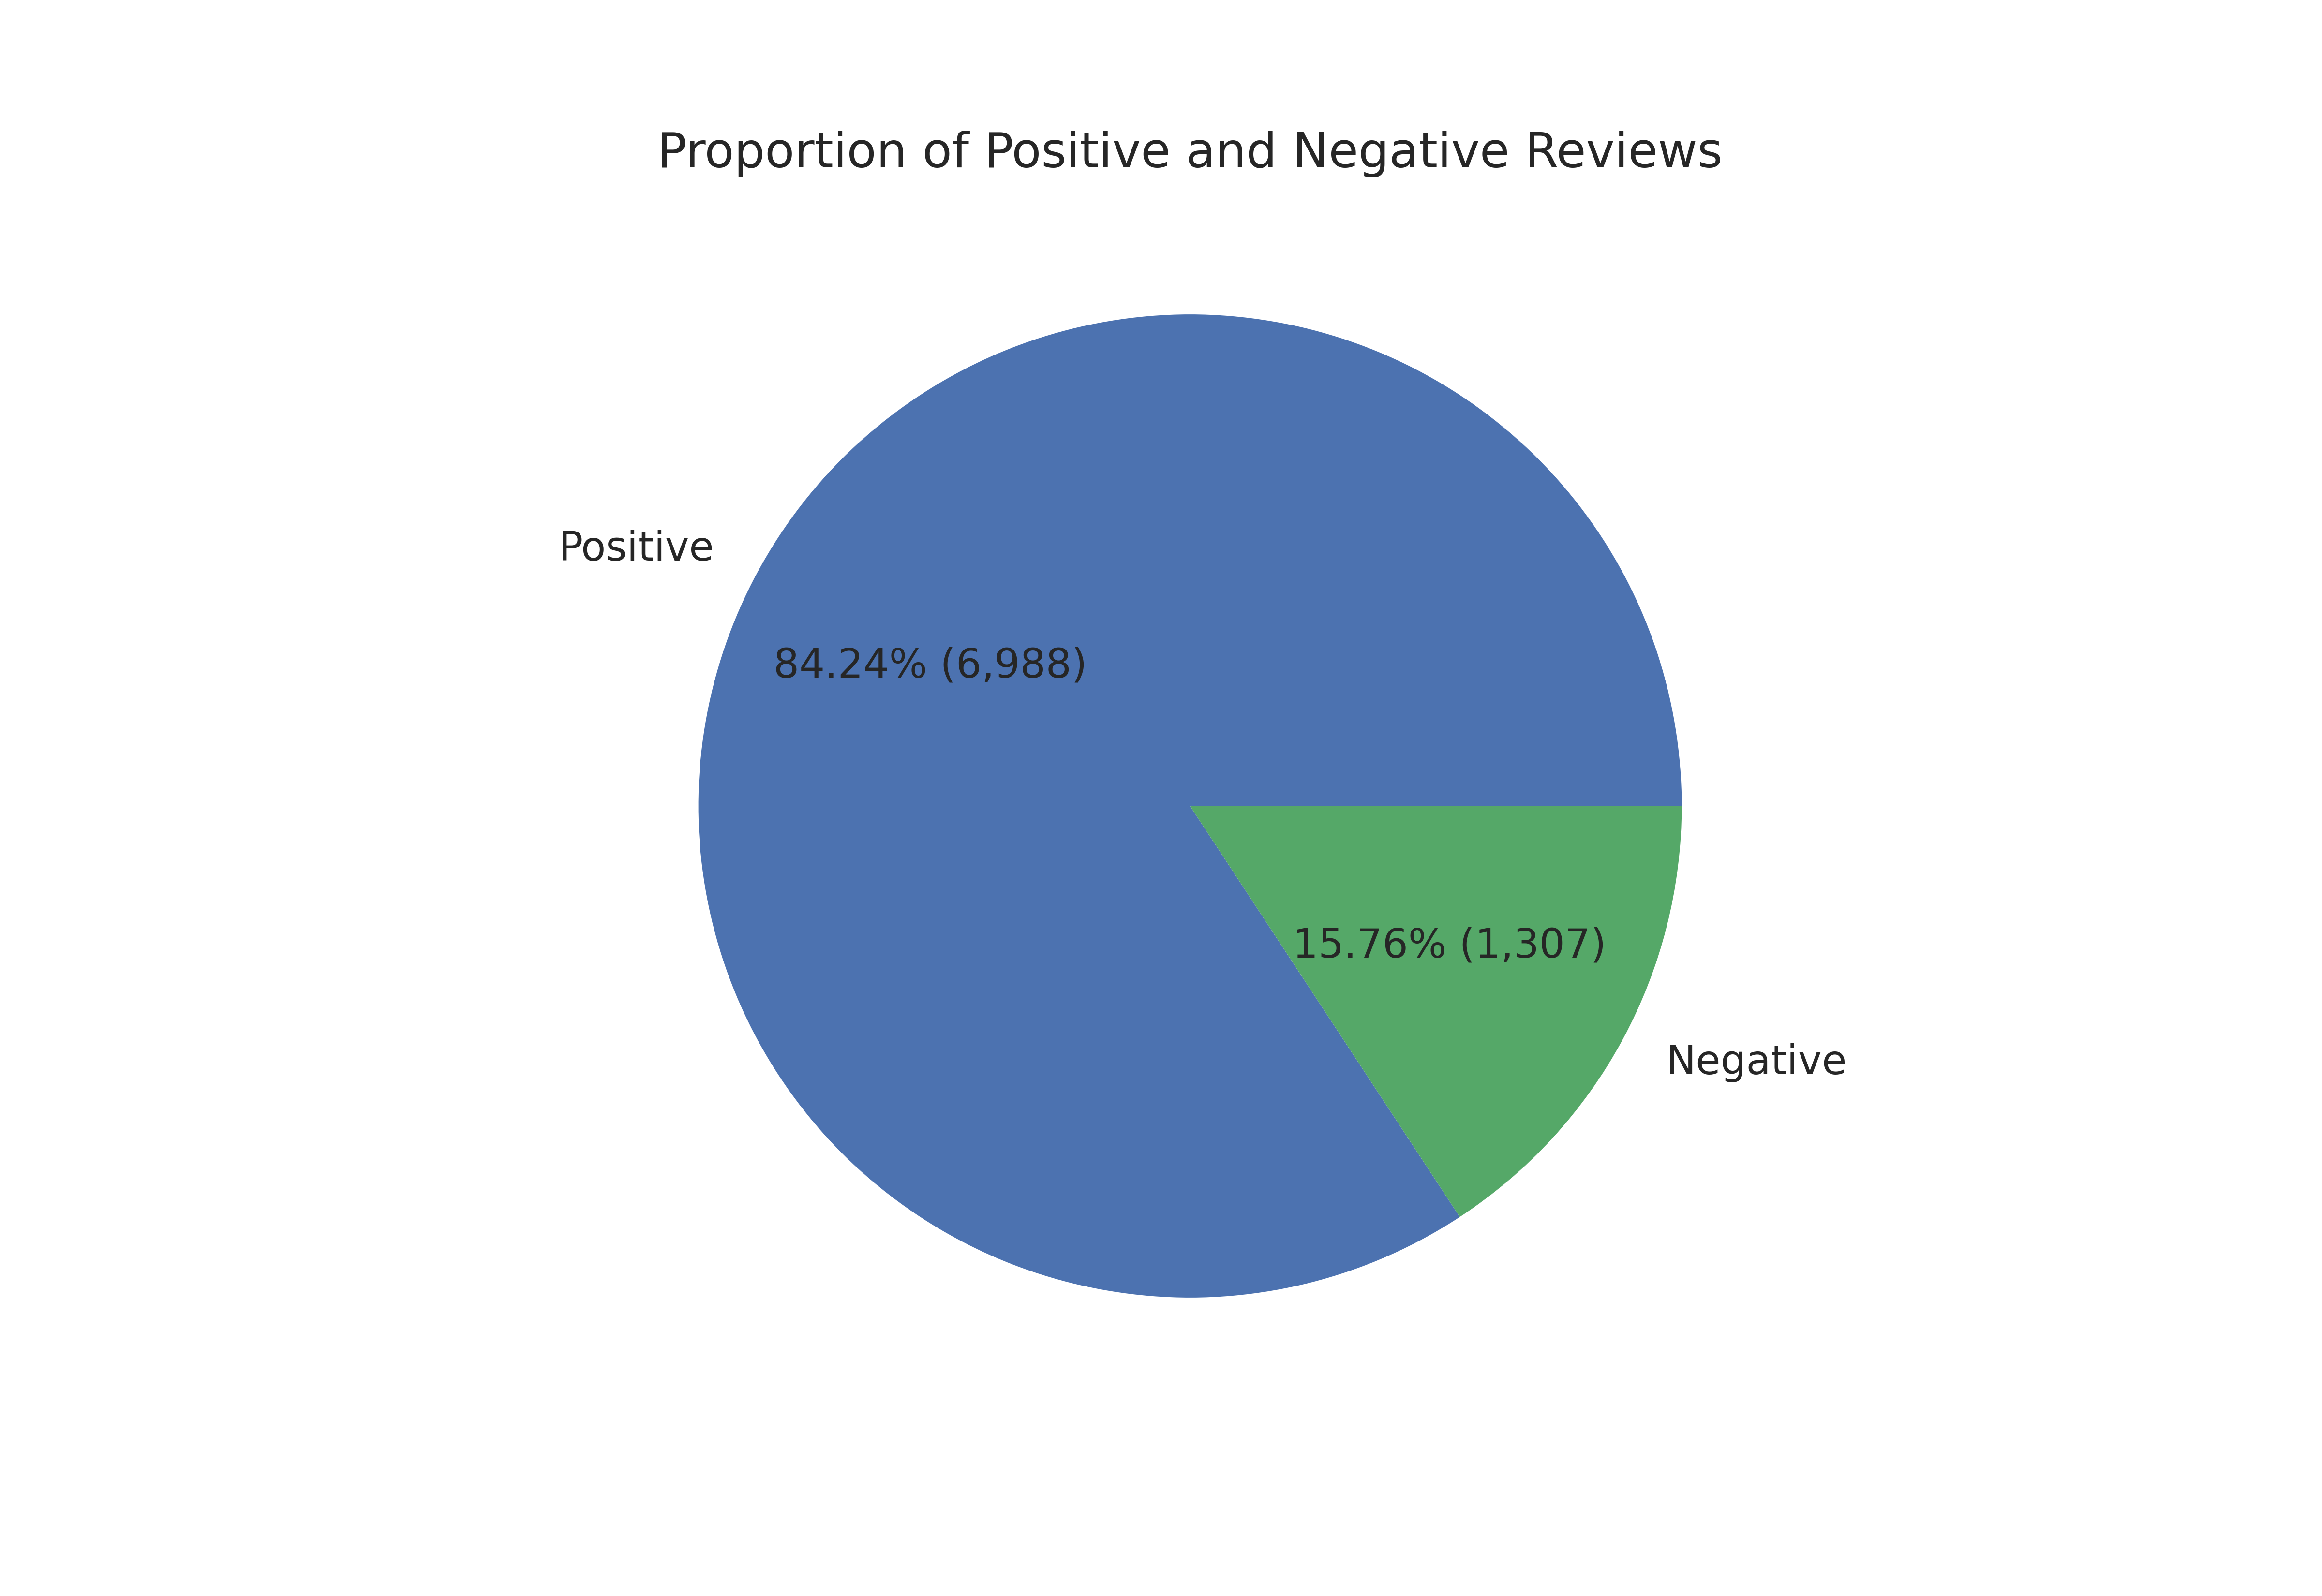
\includegraphics[width=0.6\textwidth]{rq2/pie_chart_2part.png}
% 	\end{center}
% 	\caption{Proportion of reviews (positive v. negative)}
% 	\label{fig:reviews-pie4}
% \end{figure}

% The hotel reviews have been quantified by sentiment into three distinct categories:
% positive, neutral and negative. It was observed that, unlike in RQ1, a large proportion
% of the reviews (\qty{70}{\percent}) are positive, with a small number of generally neutral reviews (\qty{17}{\percent})
% and an even smaller number of negative reviews (\qty{13}{\percent}).

% \subsection{RQ3: Predicting Sentiments By Token Frequency}
% Using the positive and negative scores SentiStrength had generated for
% each review, the reviews were classified into three categories: net positive,
% net neutral and net negative. Only net positive and net negative reviews were
% considered for this prediction.

% A frequency table for each token was generated, which shows
% how often a token of each net score appears in the entire dataset
% of hotel reviews. The distribution of reviews (based on score and
% polarity) is represented in the graph below. The horizontal axis represents
% the overall sentiment score (a whole number, from \num{-5} to \num{5}) of a review,
% and the vertical axis represents the count of tokens of that sentiment score.

% \begin{figure}[htpb]
% 	\begin{center}
% 		\includegraphics[width=0.95\textwidth]{rq3/distribution.png}
% 	\end{center}
% 	\caption{Frequency distribution of tokens by sentiment score}
% 	\label{fig:hist}
% \end{figure}

% \subsubsection{Logistic Regression Model}
% A \bf{logistic regression model} was constructed to predict whether the sentiment
% of a hotel review was either positive or negative. A logistic regression model
% is a type of statistical model used for binary classification tasks, where the goal
% is to predict the probability that an instance (in this case, a review) belongs to one of two classes---in
% this case, net positive sentiment and net negative sentiment (\(1\) and \(-1\) respectively).

% The precision-recall graph was plotted, which illustrates the proportion of positive
% predictions the model can accurately make.

% \begin{figure}[htpb]
% 	\begin{center}
% 		\includegraphics[width=0.95\textwidth]{rq3/prec-recall_logreg.png}
% 	\end{center}
% 	\caption{2-class precision-recall curve of logistic regression model}
% 	\label{fig:lg-prcurve}
% \end{figure}

% The average precision of the model is \num{0.80}, hence the model is quite accurate
% according to statistical norms.

% The receiver operating characteristic (ROC) curve of the logistic regression model
% was also plotted. The higher the ROC curve is positioned over the straight line, the higher
% the sensitivity of the model---its ability to identify true positive instances---and
% thus the accuracy of the model.

% \begin{figure}[htpb]
% 	\begin{center}
% 		\includegraphics[width=0.95\textwidth]{rq3/roc_logreg.png}
% 	\end{center}
% 	\caption{Receiver operating characteristic curve of logistic regression model}
% 	\label{fig:lg-roc}
% \end{figure}

% The area under the ROC curve (AUC) measures the ability of the model to
% distinguish between true positive and false positive instances. It ranges
% from \(0\) to \(1\), where \(1\) indicates the perfect separation of the two classes
% (true positive and false positive predictions), while \(0\) indicates that the two classes
% are indistinguishable for the model. A higher AUC value indicates more accurate model
% performance; it is able to distinguish between positive and negative instances to a
% larger extent. For this ROC curve, the AUC is \num{0.70}, hence the logistic regression model
% performs well at distinguishing true positive and false positive predictions.

% \subsubsection{Random Forest Classifier}
% A \bf{random forest classifier} was also constructed to predict
% whether hotel reviews carry a net positive or negative sentiment.
% A random forest classifier relies on feature importance---how important a feature of
% the dataset, the individual tokens which carry sentiment---are in making future predictions.
% The model takes random samples from the dataset of hotel reviews, then generates
% multiple decision trees, after which it consolidates the results from each decision tree.
% By comparing its predictions with the results obtained, the precision of the model can be
% determined.

% \begin{figure}[htpb]
% 	\begin{center}
% 		\includegraphics[width=0.95\textwidth]{rq3/prec-recall_rf.png}
% 	\end{center}
% 	\caption{2-class precision-recall curve of random forest classifier}
% 	\label{fig:rf-prcurve}
% \end{figure}

% From the precision-recall curve that was plotted, the average precision
% of this model is \(0.68\), thus the model can be said to be quite accurate.

% \begin{figure}[htpb]
% 	\begin{center}
% 		\includegraphics[width=0.95\textwidth]{rq3/roc_rf.png}
% 	\end{center}
% 	\caption{Receiver operating characteristic curve of random forest classifier}
% 	\label{fig:rf-roc}
% \end{figure}

% For the ROC curve of the random forest classifier, the AUC is \(0.91\), hence
% the random forest classifier performs well at distinguishing true and false
% positive predictions.

% \section{Discussion and Further Extension}
% Throughout this project, sentiment analysis was performed on a dataset of
% international hotel reviews in English. Hotel reviews were tokenised---split
% into individual words which carry their own meaning---and their sentiments
% determined using a sentiment lexicon. Although the majority of the lexicon
% contains neutral tokens, the number of tokens that carry positive sentiment
% far exceeds that with negative sentiment. On a larger scale, the sentiments
% of individual hotel reviews were quantified using SentiStrength with two scores:
% a positive and a negative sentiment score. The hotel reviews were then classified
% into three polarities: net positive, net neutral and net negative. A logistic
% regression model, which relies on a sigmoid function to evaluate the probability
% of a review being positive, and a random forest classifier, which relies on multiple
% decision trees created using different random subsets of the data---in this case, the
% frequency of each token, were created to predict the sentiments of hotel reviews. Upon
% making predictions, the models were found to have average precisions of \(0.80\) and \(0.68\)
% respectively, and a high rate of success in distinguishing false positive
% and true positive predictions.

% There are a few limitations to this project. Homographs---words that have the same spelling
% but different meanings---could not be distinguished during tokenisation (RQ1), resulting in
% slightly unreliable sentiment scores assigned. For example, the word \it{lobby} was shown to
% have a negative sentiment, as seen in the word cloud generated for negative tokens, although
% in context, the word \it{lobby} was used to refer to a hotel's lobby, rather than a group of
% people seeking to influence legislators on a particular issue. Furthermore, the data collected
% was limited only to English international hotel reviews, whereas some of the literature that was
% referred to managed to expand this to other languages. A more complete analysis of hotel reviews
% would include tourists of different language backgrounds, and hence sentiment analysis would need
% to be conducted in more than one language. Lastly, while a random forest classification generally
% gives more diverse results via random selection of token frequencies, it fails to discover trends
% that would enable it in extrapolating values that fall outside the training data,
% since it relies on the average of all the results of its decision trees instead. Furthermore,
% a logistic regression model assumes that the \it{tf-idf} values of tokens and the overall sentiment
% of a review are linearly related, which may hinder the accuracy of the predictions it makes.

% Much can be done to extend this project, because of the relatively small scale on which this project
% was conducted. As above, sentiment analysis could be conducted in more than one language (besides English),
% to gain a broader understanding of tourists' preferences in hotels from different languages and cultural
% backgrounds. Furthermore, more prediction models could be constructed. This would create a larger
% variation in the predictions made, enabling the precision of the models used in this project to be
% compared with those of other models to evaluate the model with the highest accuracy. Constructing a
% wider range of prediction models also allows for the possibility of more advanced techniques,
% including Naïve-Bayes prediction models or Recurrent Neural Networks (RNN), both of which are
% widely used in analysing sentiment from textual data.

% \printbibliography

% \begin{singlespace}
% 	\section{Appendices}

% 	\subsection{RQ1 Source Code}
% 	\pycode{../../code-ready/rq1_report.py}

% 	\subsection{RQ2 Source Code}
% 	\pycode{../../code-ready/rq2_report.py}

% 	\subsection{RQ3 Source Code: Logistic Regression}
% 	\pycode{../../code-ready/rq3_logreg_report.py}

% 	\subsection{RQ3 Source Code: Random Forest Classifier}
% 	\pycode{../../code-ready/rq3_randomforest_report.py}
% \end{singlespace}

\end{document}
